\chapter{Systems}
\label{ch:system}
\section{Introduction}
In this section, we will discuss the hardware and software implementation of our complete system setup. First, we will begin with hardware setup encompassing the sensors and platforms utilized for data collection. Next, we will show the details of implementations of our complete system in three different operating modes: online SLAM, offline multi-mission SLAM map merging, and relocalization within ROS framework. In all those three modes, the place recognition server module provides loop closure information. VILENS odometry is used as the base state estimation module in online SLAM and relocalization, and VILENS SLAM module is used in online SLAM mode managing pose graph. 

\begin{figure}[htbp]
  \centering
  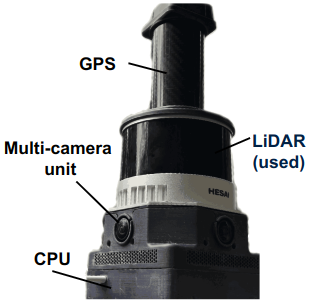
\includegraphics[width=0.4\columnwidth]{pics/setup_Frontier_pic2.png}
  \caption{Image of \emph{Frontier} device comprising a LiDAR, IMU, three cameras, GPS and CPU board. }
  \label{fig:frontier}
\end{figure}

\section{Hardware Setup}
\label{sec:system_setup}
We use a multi-sensor unit called \emph{Frontier}, which comprises a LiDAR, IMU, three cameras and onboard CPU computing (additionally GPS) shown in \figref{fig:frontier}. We used two different \emph{Frontier} device, \emph{Frontier-15} and \emph{Frontier-19} which contains Hesai XT-32 and Hesai QT-64 LiDAR respectively and the details of sensor specifications are summarized in \tabref{tab:sensors}. For the different \emph{Frontier} devices, we modify configuration settings on both VILENS odometry and VILENS SLAM (details in \cite{wisth2023tro,proudman2022ras}). For data collection, we mainly used human and legged robot platforms as shown in \figref{fig:system_setup}. We typically mapped the forest area in zigzag patterns to ensure coverage in both forward and backward. 



\begin{table}[t]
  \centering
  \small
  \begin{tabular}{|c|c|>{\raggedright\arraybackslash}p{4.5cm}|}
      \hline
      \multicolumn{1}{|c|}{\textbf{Sensor Type}} & \multicolumn{1}{|c|}{\textbf{Name}} & \multicolumn{1}{|c|}{\textbf{Characteristics}} \\
      \hline
      \multirow{8}{*}{LiDAR} & \multirow{4}{*}{Hesai Pandar XT-32 (\emph{Frontier-15})} & \textbullet\, 10 Hz \newline \textbullet\, 360° × 31° FoV \newline \textbullet\, 0.18° × 1° Res. \newline \textbullet\, 0.5--120 m Range \\
      \cline{2-3}
      & \multirow{4}{*}{Hesai Pandar QT-64 (\emph{Frontier-19})} & \textbullet\, 10 Hz \newline \textbullet\, 360° × 104° FoV \newline \textbullet\, 0.6° × 1.45° Res. \newline \textbullet\, 0.1--60 m Range \\
      \hline
      \multirow{4}{*}{Cameras} & \multirow{4}{*}{Sevensense, Alphasense} & \textbullet\, 30 Hz \newline \textbullet\, 126° × 92.4° FoV \newline \textbullet\, RGGB Bayer Fisheye \newline \textbullet\, 1440×1080 pixels \\
      \hline
      \multirow{2}{*}{IMU} & \multirow{2}{*}{Bosch BMI085} & \textbullet\, 400 Hz \newline \textbullet\, 6-axis \\
      \hline
      \multirow{1}{*}{GNSS} & \multirow{1}{*}{U-blox} & \textbullet\, CNR:30-50 dB  \\
      \hline
  \end{tabular}
  \caption{Sensor specifications of \emph{Frontier} multi-sensor unit device.}
  \label{tab:sensors}
\end{table}



\begin{figure}[htbp]
  \centering
  \includegraphics[width=0.70\columnwidth]{pics/setup_4yp_platform_fig3.pdf}
  \caption{Platform setup for forest mapping. Backpack (shown in left) with \emph{Frontier} mounted for a human mapping scenario, and a legged robot (shown in right) for forest surveying and monitoring applications.}
  \label{fig:system_setup}
\end{figure}


\section{Implementations}
\label{sec:implementation}
\subsection{Robotic Operating System (ROS) Framework}
The Robot Operating System (ROS) is a flexible framework for developing software for robotics applications as shown in \figref{fig:implementation_ros}. One of the key concepts in ROS is the publisher-subscriber model, where nodes (independent processes) communicate by publishing messages on topics and subscribing to messages on those topics. Publishers broadcast data, such as sensor readings or robot state information, while subscribers receive and process these data. The nodes and published topics then estalbish a network that represents the data sharing; this can be visualized with ROS tools such as \emph{rqt graph} as shown in \figref{fig:implementation_ros}. Additionally, ROS facilitates communication between nodes through service calls and servers. Services allow nodes to request specific tasks or information from one another, where the client sends a request message and the server responds accordingly, enabling more complex interactions beyond simple message passing shown in service call box in \figref{fig:implementation_ros}. This modular and distributed architecture of ROS makes it well-suited for building modular and scalable robotic systems. 
\begin{figure}[htbp]
  \centering
  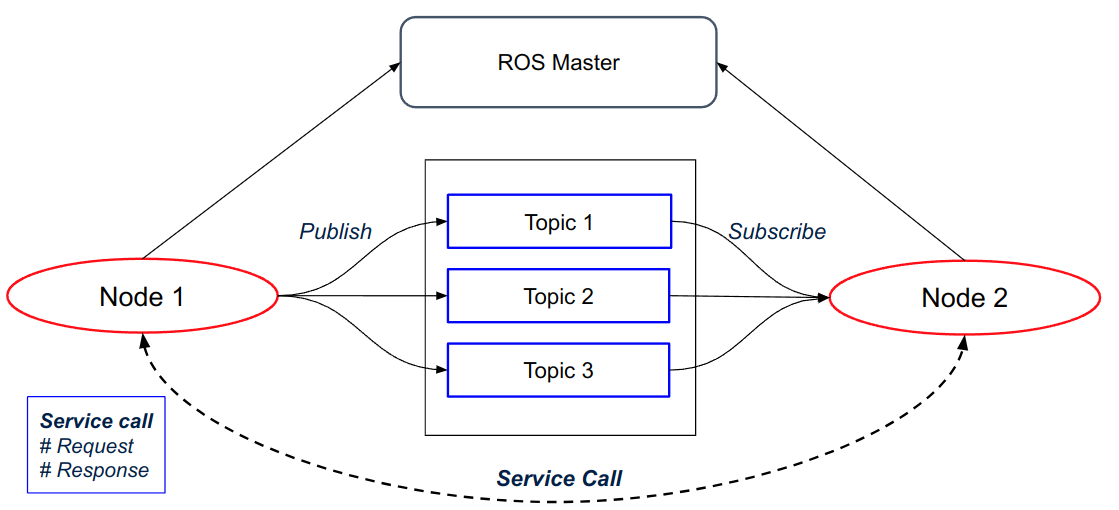
\includegraphics[width=0.8\columnwidth]{pics/Implementation_ros_framework2.png}
  \caption{ROS Framework. Nodes are shown in red elipses, published topics are shown in blue boxes. Additionally, we also define service call, a client node requests a specific service message and a server node responses a service message based on request. Edges are connections between nodes.}
  \label{fig:implementation_ros}
\end{figure}

\subsection{Online SLAM}
This is a basic setup for single mission SLAM. Previosuly, place recognition model \emph{Scan Context}, was directly integrated inside VILENS SLAM. But now, place recognition server acts like a separate module and is shown in \figref{fig:implementation_online_slam}. The place recognition server subscribes to LiDAR scan and pose graph topics from VILENS SLAM. The place recognition server then publishes service messages to VILENS SLAM node. Service message contains the loop candidate information including candidate id and relative transformation. The overall online SLAM nodes and topics used are shown in \figref{fig:implementation_online_slam}. 

\begin{figure}[htbp]
  \centering
  \includegraphics[width=0.99\columnwidth]{pics/Implementation_Online_SLAM_redraw3.pdf}
  \caption{Online SLAM Implementation. Loop closure candidates information is transmitted to VILENS SLAM node from the place recognition server node. This occurs whenever new LiDAR point clouds comes in to the place recognition server node from VILENS SLAM node. }
  \label{fig:implementation_online_slam}
\end{figure}


\subsection{Offline Multi-mission SLAM Map Merging}
Offline Multi-mission SLAM maps merging runs in post-processing. Loop closure requests and detections are transmitted between VILENS SLAM Offline node and the place recognition server node via service calls. From VILENS SLAM Offline node individual point clouds, cloud ids of a mission and pose graph can be used as input to place recognition server node. The place recognition server node builds the descriptor database incrementally mission by mission. Then, when it finds loop closures it makes service calls back to VILENS SLAM Offline node. The overall offline multi-mission SLAM nodes and topics used are shown in \figref{fig:implementation_offline_slam}.  

\begin{figure}[htbp]
  \centering
  \includegraphics[width=0.89\columnwidth]{pics/Implementation_Offline_SLAM_redraw_2.pdf}
  \caption{Offline multi-mission SLAM map merging implementation. For each mission, every input point clouds are passed to the place recognition server node to find loop closures. The place recognition server node then makes a service call back to VILENS SLAM Offline node.}
  \label{fig:implementation_offline_slam}
\end{figure}


\subsection{Relocalization}
The relocalization application showcases the use of the place recognition server when a complete prior map is available. As shown in \figref{fig:implementation_relocalization}, the VILENS SLAM node is replaced by the place recognition client node, which stores the prior map's individual point clouds, pose graph, and descriptors. Similar to the online SLAM mode, the place recognition server node processes the incoming sensor data and extracts descriptors to search for loop closure candidates against the prior map's descriptors. However, unlike the Online SLAM mode where the VILENS SLAM node performed pose graph optimization, the place recognition server does not perform this optimization. Instead, it simply sends the detected loop closure messages to the place recognition client node. The place recognition client node then uses these loop closures to relocalize and visualize the current robot's pose within the prior map's coordinate frame, without modifying the prior map itself.

In order to visualize the pose of the robot continuously, we need to complete the transformation tree between \emph{map} and \emph{odom} frames shown in \figref{fig:implementation_relocalization_tf}. Transformation tree is a hierarchical structure that manages coordinate frame transformations in ROS. This follows two steps: when loop closures are verified from place recognition server, we can compute transformation between \emph{map} and \emph{base}. Then from VILENS odometry, we access transformation between \emph{base} and \emph{odom}. We then compute the transformation between \emph{map} and \emph{base} then publish as transformation message. Now this verified transformation is synchronized with VILENS odometry to visualize the pose of the robot. Whenever new loop closures are verified, we change current transformation between \emph{map} and \emph{odom} and republish as transformation message. With localization now expressed with respect to the prior map we can demonstrate this utility by creating a virtual visualization of
the forest from the perspective of a camera mounted with the LiDAR sensor.

\begin{figure}[htbp]
  \centering
  \includegraphics[width=0.99\columnwidth]{pics/Implementation_Relocalization_redraw_3.pdf}
  \caption{Relocalization implementation. Similar to Online SLAM mode, place recognition server node provides a loop closures message to the place recognition client node. The place recognition client node then continuously publishes transformation to relocalize the current robot's pose in map frame. Finally, robot pose, camera images and virtual tree models can then be drawn in visualization node.}
  \label{fig:implementation_relocalization}
\end{figure}



\begin{figure}[htbp]
  \centering
  \includegraphics[width=0.99\columnwidth]{pics/implementation_tf_trees4.pdf}
  \caption{Transformation tree in relocalization mode. Transformation between \emph{map} and \emph{odom} frames should be connected by two steps. First, getting transformation between \emph{map} and \emph{base} from the place recognition server then use most recent transformation between \emph{base} and \emph{odom} from VILENS odometry to compute target transformation between \emph{map} and \emph{odom}.}  
  \label{fig:implementation_relocalization_tf}
\end{figure}